\documentclass{bioinfo}
\copyrightyear{2015} \pubyear{2015}

\access{Advance Access Publication Date: Day Month Year}
\appnotes{Manuscript Category}

\begin{document}
\firstpage{1}

\subtitle{Really cool deep learning stuff}

\title[short Title]{General purpose gene annotation using deep learning}
\author[Sample \textit{et~al}.]{Felix Stiehler\,$^{\text{\sfb 1,}}$$^\dagger$, Alisandra Denton\,$^{\text{\sfb 1,}}$$^\dagger$\, Marvin Steinborn\,$^{\text{\sfb 1}}$, Stephan Scholz, Andreas Weber\,$^{\text{\sfb 1,}*}$}
\address{$^{\text{\sf 1}}$Institue for Plant Biochemistry, Heinrich-Heine-University, Dusseldorf, D-40225, Germany}

\corresp{$^\dagger$Authors contributed equally. \newline $^\ast$To whom correspondence should be addressed.}

\history{Received on XXXXX; revised on XXXXX; accepted on XXXXX}

\editor{Associate Editor: XXXXXXX}

\abstract{\textbf{Motivation:} Current state of the art gene annotation programs for eukaryotic genomes have to be pretrained for each species and still often produce annotations that lack the required accuracy. \\
\textbf{Results:} We set up a framework that can be used to build much more general gene callers that also outperform traditional methods on a variety of complex genomes.\\
\textbf{Availability:} Text  Text Text Text Text Text Text Text Text Text  Text Text Text Text
Text Text Text Text Text Text Text Text Text Text Text Text Text Text  Text\\
\textbf{Contact:} \href{name@bio.com}{name@bio.com}\\
\textbf{Supplementary information:} Supplementary data are available at \textit{Bioinformatics}
online.}

\maketitle

\section{Introduction}
\begin{itemize}
	\item Calling genes correctly is very important
	\item but also very difficult in eukaryotes
	\item All current state of the art gene callers work based on HMMs
	\item The structure of the HMMs is finely tuned and engineered
	\item Actual learning is very limited, and with that generalization across different genomes 
	\item (Also have problems with genes that contain long introns, common in mammals)
\end{itemize}

\section{Approach}
Helixer is a prototype software for training and utilizing a general purpose model for the functional annotation of large eukaryotic genomes. We demonstrate the effectiveness of this approach by training a single model for animals (phylogenetic names?) and plants respectively, which was then evaluated on 192 genomes in the animal case and on 60 plant genomes. We use modelling techniques from the field of deep learning, which has been shown to have the potential to be superior in flexibility and accuracy to traditional machine learning methods in a variety of fields. Our model expects the raw genomic sequence as main input and produces functional predictions on a base pair wise level. The source code and all data is publically available.

\begin{methods}
\section{Methods}
	We worked with 192 animal and 60 plant genomes. The data of each genome consists of the latest publically available genomic assembly in form of a FASTA file and the latest annotation in the GFF format. We used all animals genomes in EnsemblMetazoa 45 (?) \citealp{Howe19} as well as those of all non-embargoed plant genomes of the JGI Phytosome 13 database (?, citation). Both data groups were used seperately during training as well as during evaluation. At the start of our work we split both genome groups into training and test sets. The test sets contained 19 or 6 genomes, respectively. The test genomes were chosen to be of the best possible quality (?) based on collected metadata while also representing a broad phylogenetic spread. Some of the remaining genomes were used for training purposes and all were used for evaluating our models. We call the genomes that were ultimatily used during training the {\it training genomes} and the remaining non-test genomes the {\it validation genomes}.

We pre-processed and stored the genomic information by using Geenuff \citealp{Denton19}. Geenuff is a tool for checking and exploring genomic data, which stores all information inside a SQL database. Training and evaluation data was generated by querying this database and transforming the returned data into a numerical format suitable for machine learning. In the case of unambiguous input data, the genomic sequence was transformed into matrix that represents a one hot encoding with 4 rows. For the other case see Supplementary material .. (). The annotations are also transformed into a 4-row one hot encoding matrix, where a one in each of the rows represents one of the possible classes {\it Intergenic}, {\it UTR}, {\it CDS} or {\it Intron}. An non-coding intron can be inferred from the prediction order. A full description of all generated data arrays can be found in table \ref{tab:arrays}.

The classes are not balanced equally and the tradeoff between the number of intergenic and intronic bases is quite different in both groups of genomes. Table \ref{tab:statistics_all} shows the ratio of class occurences, together with other overall metrics.

\begin{table}[!t]
\processtable{Data group statistics for all data\label{tab:statistics_all}} {
\begin{tabular}{@{}lll@{}}
\toprule & Animals & Plants\\
\midrule
Average genome size in Gbp& 2.936 (+- 1.562) & 0.787 (+- 0.995) \\
Average gene length & 31,223 (+- 13,974)& 3,368 (+- 1,510)\\
Geenuff error rate & 0.311 (+- 0.129) & 0.351 (+- 0.249) \\
Fraction of class Intergenic  & 0.777 (+- 0.042) & 0.799 (+- 0.089) \\
Fraction of class UTR & 0.006 (+- 0.006) & 0.017 (+- 0.016) \\
Fraction of class CDS & 0.016 (+- 0.014) & 0.085 (+- 0.071) \\
Fraction of class Intron & 0.201 (+- 0.035) & 0.099 (+- 0.057) \\
\botrule
\end{tabular}}{Values are averages of the individual values of each genome in a data group. All statistics except the average gene lengths are excluding FASTA sequences without a gene and subsequences that were masked as completely erroneous. Each strand of DNA was counted seperately. The average gene length was determined by the average length of the longest transcript by cumulative exon length, which is how we query for genes during data generation. Brackets show the standart deviation.}
\end{table}

During data generation, we only queried for the longest transcript of each gene and did not include FASTA sequences that had no functional annotation (explanation why this is a sign of error?). As Geenuff checks the genomic annotations for potential errors and is able to mark those areas, we were able to effectively blank out those bases during training. The vast majority of bases masked lie in the intergenic region as the most prevelant error is a missing UTR and Geenuff marks a potentially large intergenic region for it. Table \ref{tab:statistics_all} shows statistics about the masking. The corresponding statistics for the selected training genomes only can be found in Section \ref{sec:training_data}. 
	
For the training, we divided each continous genomic sequence into 20.000 bases long subsequences, which are then used as input or label for the neural network. We appended zero padding if the subsequences are not long enough. If a subsequence is fully marked as erroneous, we do not include it anywhere.

The selection of training genomes requires balancing multiple conflicting tradeoffs. On the one hand, we do want to train with as much data as possible, but not all data has a good enough quality to enable a powerful generalization. It is also very desirable to have a broad spread in phylogenetic distance as well as genome size and average gene length as the model is increasingly unlikely to generalize well beyond the borders given by the training data. However, if the genomic patterns inside the data are too different from each other, it may be difficult for the model to generalize as well. It was also important to us to get experimental results within a couple of days as we tested many different data and model configurations, which limited the overall size of the training set and the model. 
	
We employed an iterative approach to effectively select a proper set of training genomes. We first started with 3-4 genomes that were almost certain to be of the highest quality. We then evaluated the performance of the resulting model on all genomes individually (including the training genomes) and looked for candidates to add to the training set or to remove from it. This process was repeated multiple times concurrently with the model search until we saw no more room for substantial improvement given our computational constraints.

Once a set of training genomes was selected, we split it up again into a {\it training and validation set}. This split of the training genomes was done to get a quicker sense of the generalization capabilities and was used primarily during training. We split of the validation set by selecting 20\% of the FASTA sequences above and below the N90 of each training genome, ensuring a proper distribution of large and short sequences in both sets and a split on the chromosome level. Evaluation of the annotations on all training and validation genomes was done regularly after a promising model candidate was found based on its validation set performance. Ultimately we only cared about the cross-species performance of a model.

We use metrics two metrics to judge model performance. The {\it Genic F1} is our primary metric that provides the most comprehensive picture of annotation quality in one number. The {\it Subgenic F1} is similar to the Genic F1, except that it does not take UTR predictions into account. This is done for comparability with Augustus and further explained in Chapter \ref{augustus}. Both metrics work by summing up True Positives (TP), False Positives (FP) and False Negatives (FN) of each considered class before calculating precision and recall from these values and combining the two into a F1 score. Both metrics do not take the values of the intergenic class into account, as this class is very abundant and appears to be by far the easiest to predict. In the case of the Genic F1, this means that effectively only the TP of the intergenic class are disregarded. The metrics essentially provide a weighted mean of the performances in the considered classes. All individual class performances are reported in Supplementary Material (?). 
	
\subsection{Model Architecture and Usage}
\label{sec:model}
We use a 4-layer deep stacked BLSTM network with 256 units per layer and layer normalization (citation ? ) between each BLSTM layer to produce the predictions in the form of a base pair wise classification. The model consists of circa 5.4 million parameters and was implemented with the deep learning library keras (citation) on top of TensorFlow (citation). We tested multiple different architectures before arriving at this model configuration, including convolutional neural networks (CNN) and hybrid architectures. The hyperparameters were determined by a combination of manual and automatic hyperparameter optimization (talk about TPE?, quote nni?). All relevant hyperparameters can be found in Table \ref{tab:params} or in the Helixer source code repository. 

We also implemented a dilated CNN (dCNN) baseline as this kind of architecture is widely used when working with DNA data as input. Details of the neural architecture search are given in Section \ref{sec:dcnn}.
	
Our final model was trained with 10 bases of genomic sequence as input during each time step and produces individual predictions for each of those 10 bases simultaneously. This grouping enabled us to train effectively with far longer sequences than usual. A class wise evaluation including the calculation of the Genic F1 score is performed on the validation set after every epoch.

We also used multiple techniques to improve the prediction quality after the training was done. One very effective way for genomes with larger genes was to input longer sequences during inference time than during training. This was done for all animal genomes except the invertebrates. The input sequences were up to 10 times larger, depending on species group and assembly quality. This also demonstrates ability of our model to generalize as it is able to make successful prediction on far longer sequences than it has ever seen. The sequence length during inference can be any of 20.000, 50.000, 100.000 or 200.000 and is determined by the species family(?). Families that tend to have longer genes get assigned longer sequences. For more implementation details on this see Section \ref{sec:longer} or the source code.
	
The final predictions of a single model are constructed by overlapping predictions, that were made from a sliding window and then cut to a core sequence. This was done to strongly reduce a typical drop in performance of the models towards the beginning and end of each sequence (see figure \ref{fig:length_wise_bias}) and also to improve model performance in general by providing the model with multiple different starting points. The different overlapping sequences were recombined by averaging the individual softmax values of each base. Supplementary Material (?) contains the influence on overlapping with respect to the position in a sequence for each genome, ordered by N75. We found that overlapping works best if the genomes are not very fragmented.

A model ensemble with 8 components was used to generate the final predictions for each species. For this, we trained 4 seperate animal and plant models and also used a model from an epoch that did not have the highest Genic F1 on the validation set. Depending on the results, we used the model iteration with either the highest genic recall or precision. The model with the best Genic F1 was always best in one of those. This was done to increase the diversity of the model ensemble. As with the overlapping, the fusion of the 8 individual predictions was done by averaging the softmax values of each base pair prediction.

\subsection{Evaluation of Augustus} \label{augustus}
What Marvin did, why we don't use Genic F1 for comparison, etc


\begin{table}[!t]
\processtable{Data arrays generated and used by Helixer\label{tab:arrays}} {
\begin{tabular}{@{}ll@{}}
\toprule Name & Information \\
\midrule
Input & Genomic sequence in a one hot encoding\\
	  & for (A, T, C, G), otherwise different, see suplementary .. ()\\
Output & Labels in a 4-dimensional one hot encoding \\
Sample weights & One of $\{0,1\}$; whether there is an error at a base\\
\botrule
\end{tabular}}{}
\end{table}

\end{methods}

\begin{figure}[!tpb]
	\centerline{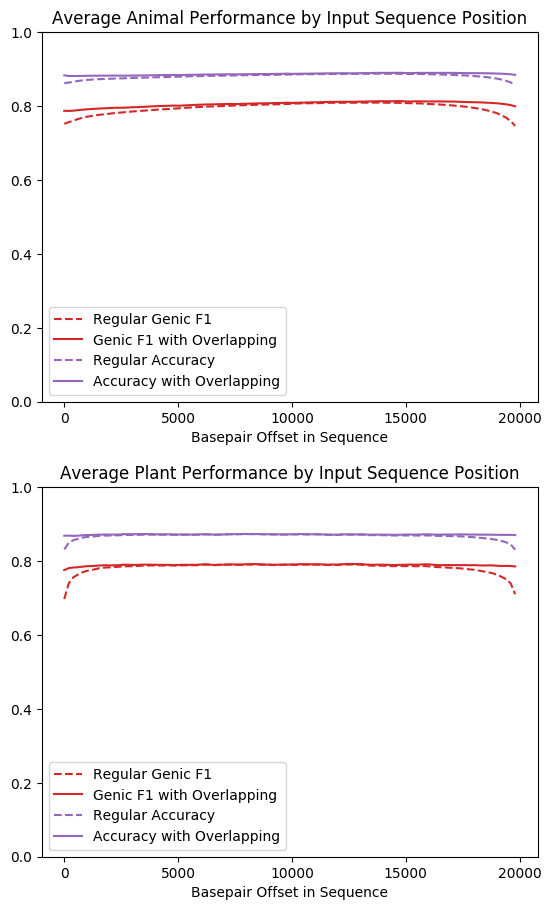
\includegraphics[width=0.45\textwidth]{images/length_wise_bias}}
\caption{Caption, caption.}\label{fig:length_wise_bias}
\end{figure}

\begin{table}[!t]
\processtable{Experimental Results and Comparison\label{tab:results}} {
\begin{tabular}{@{}lll@{}}
\toprule & Animals & Plants\\
\midrule
Augustus & 0.632 (+-0.089) & 0.749 (+-0.161)\\
Dilated CNN Baseline & - (+-) & - (+-)\\
Best Helixer model & - (+-) & - (+-) \\
Best model + varied input length & - (+-) & - \\
Best model (+ varied input length) + overlapping &  0.85 (+-0.068) & 0.843 (+-0.151) \\
(Varied input length +) overlapping + ensembling & 0.868 (+-0.064) & 0.863 (+-0.148) \\
\botrule
\end{tabular}}{Values are the median in Subgenic F1 across all validation and test genomes of the respective group. Varied input length was only used in the animal case. The best model was chosen out of the eight models of the ensemble for having the best performance in the reported setup. The Augustus result is the median score for all genomes.}
\end{table}

\section{Results}
We evaluate our performance based on the average cross-species Subgenic F1 for all genomes except the few used during training. The results are displayed in Table \ref{tab:results} and show a clear improvement over the AUGUSTUS and dilated CNN baselines. We also demonstrate the effectiveness of two techniques used during inference with the usage of longer input lengths being enabled by our LSTM stack without any fully connected layers on top. To our knowledge, this technique was not used before with a model used for gene annotation.

\section{Conclusion}
We propose a gene calling model that is able to perform cross-species genomic annotiation for a wide variety of large eucaryotic genomes. Our model does this while outperforming AUGUSTUS on a base pair wise level and withstanding RNASeq data based scrutiny. 

\section*{Acknowledgements}

We are very grateful for the support of...

\section*{Funding}

This work has been supported by the... Text Text  Text Text.\vspace*{-12pt}

%\bibliographystyle{natbib}
%\bibliographystyle{achemnat}
%\bibliographystyle{plainnat}
%\bibliographystyle{abbrv}
%\bibliographystyle{bioinformatics}
%
%\bibliographystyle{plain}
%
%\bibliography{Document}


\begin{thebibliography}{}

\bibitem[Denton {\it et~al}., 2019]{Denton19}
Denton,A., Stiehler,F. (2019) Article title, {\it Journal Name}, {\bf 199}, 133-154.

\bibitem[Howe KL {\it et~al}., 2019]{Howe19}
Howe KL, Contreras-Moreira B, De Silva N, Maslen G, Akanni W, Allen J, Alvarez-Jarreta J, Barba M, Bolser DM, Cambell L, Carbajo M, Chakiachvili M, Christensen M, Cummins C, Cuzick A, Davis P, Fexova S, Gall A, George N, Gil L, Gupta P, Hammond-Kosack KE, Haskell E, Hunt SE, Jaiswal P, Janacek SH, Kersey PJ, Langridge N, Maheswari U, Maurel T, McDowall MD, Moore B, Muffato M, Naamati G, Naithani S, Olson A, Papatheodorou I, Patricio M, Paulini M, Pedro H, Perry E, Preece J, Rosello M, Russell M, Sitnik V, Staines DM, Stein J, Tello-Ruiz MK, Trevanion SJ, Urban M, Wei S, Ware D, Williams G, Yates AD, Flicek P. (2019) Ensembl Genomes 2020-enabling non-vertebrate genomic research. {\it Nucleic Acids Research 2019} https://doi.org/10.1093/nar/gkz890

\end{thebibliography}

\newpage

\section{Supplementary Material}

\subsection{Dilated CNN Baseline Network Search}
\label{sec:dcnn}
\begin{table}[!t]
\processtable{Parameter search space for the dilated CNN baselines\label{tab:dcnn}} {
\begin{tabular}{@{}ll@{}}
\toprule Parameter & Possible Values \\
\midrule
Kernel Size & \{4, 8, 12, 16\}\\
Initial Filter Depth & \{32, 64, 96, 128\}\\
Number of Layers Before Doubling Filter Count & \{1, 2\}\\
Dilation Multiplier & \{2, 3\}\\
Number of Convolutional Layers & \{2, 3, 4, 5, 6, 7, 8\}\\
Number of Hidden Fully Connected (FC) Layers & \{0, 1, 2\}\\	
Dropout Used on FC Output & \{0.0, 0.01, 0.1, 0.2, 0.3\}\\
Learning Rate & \{1e-3, 1e-4\}\\

\botrule
\end{tabular}}{Above are all parameters used during neural architecture search for the dilated CNN baseline. The same overall space was used for plant and animal data. We did, however, run multiple distinct searches that sometimes only operated over a subset of the given parameters. This was done as those seemed to be the most promising. We for example restricted the search space of the number of LSTM layers to the highest 3 values in later runs. Decisions were guided by the Genic F1 on the validation set of exactly the same data we trained our final LSTM models with. Run with a Genic F1 below 0.5 after 10 epochs were stopped at that point and the overall maximum epoch was 15. The batch size used for almost all runs was 32 and the dilation was capped to 81. The performances seemed to be leveling of well before that. The implementation and parameter space is very roughly based on (paper we looked at?) and can be found in the Helixer source code repository. In total, we ran (?) runs for the plant and (?) runs with the animal data.}
\end{table}

\begin{table}[!t]
\processtable{Final Parameters of dilated CNN baselines\label{tab:dcnn_best}} {
\begin{tabular}{@{}lll@{}}
\toprule Parameter & Possible Animal Values & Possible Plant Values\\
\midrule
Layers & 4 & \\
Units per layer & 256 & \\
Learning rate & 1e-4 & \\
Optimizer & Adam & \\
\botrule
\end{tabular}}{The parameters of the dilated CNN model that performed the best according to the Genic F1 of the validation data of the respective training genomes. }
\end{table}


\subsection{Input Data Encoding}


\subsection{Hyperparameters}

\begin{table}[!t]
\processtable{Hyperparameters\label{tab:params}} {
\begin{tabular}{@{}ll@{}}
\toprule Name & Value \\
\midrule
Layers & 4\\
Units per layer & 256\\
Learning rate & 1e-4\\
Optimizer & Adam\\
\botrule
\end{tabular}}{}
\end{table}

\begin{table}[!t]
\processtable{Class weights\label{tab:params_cw}} {
\begin{tabular}{@{}lll@{}}
\toprule Class & Animal Value & Plant Value \\
\midrule
[0.7, 1.6, 1.2, 1.2] & 4 &\\
\botrule
\end{tabular}}{see data statistics tables..}
\end{table}


\subsection{Training Data statistics}
\label{sec:training_data}
\begin{table}[!t]
\processtable{Data group statistics for our training data\label{tab:statistics_training}} {
\begin{tabular}{@{}lll@{}}
\toprule & Animals & Plants\\
\midrule
Average genome size in Gbp& 2.489 (+- 2.073) & 0.914 (+- 0.934) \\
Average gene length & 25,672 (+- 16,605) & 3,509 (+- 906)\\
Geenuff error rate & 0.253 (+- 0.138) & 0.134 (+- 0.072) \\
Fraction of class Intergenic & 0.752 (+- 0.05) & 0.808 (+- 0.106) \\
Fraction of class UTR & 0.013 (+- 0.011) & 0.033 (+- 0.023) \\
Fraction of class CDS & 0.028 (+- 0.028) & 0.077 (+- 0.052) \\
Fraction of class Intron  & 0.207 (+- 0.023) & 0.083 (+- 0.037) \\
\botrule
\end{tabular}}{The description of Table \ref{tab:statistics_all} applies here as well.}
\end{table}

\subsection{Longer Sequence Input}
\label{sec:longer}
Implementation detail:
If the N75 of a species is less than twice as high as the supposed sequence length it is lowered until either this criteria is met or a length of 50.000 is reached. 

Table of species with their length.



\end{document}
